\documentclass{HW}

\newcommand{\hwtitle}{آزمایش یک}
\newcommand{\studentname}{رادین شایانفر}
\newcommand{\studentnumber}{9731032}

\usepackage[top=30mm, bottom=30mm, left=25mm, right=25mm]{geometry}
\usepackage{amsthm,amssymb,amsmath,amsfonts}
\usepackage{fancyhdr}
\usepackage{changepage}
\usepackage{enumitem}
\usepackage{listings}
\usepackage[table]{xcolor}
\usepackage{fontspec}

\newfontfamily{\ttconsolas}{Consolas}

\definecolor{codegreen}{rgb}{0,0.6,0}
\definecolor{codegray}{rgb}{0.5,0.5,0.5}
\definecolor{codepurple}{rgb}{0.58,0,0.82}
\definecolor{backcolour}{rgb}{0.95,0.95,0.92}

\lstset{
  backgroundcolor=\color{backcolour},   
  commentstyle=\color{codegreen},
  keywordstyle=\color{magenta},
  numberstyle=\tiny\color{codegray},
  stringstyle=\color{codepurple},
  basicstyle=\ttconsolas\footnotesize,
  breakatwhitespace=false,         
  breaklines=true,                 
  captionpos=b,                    
  keepspaces=true,  
  numbers=left,                    
  numbersep=5pt,                  
  showspaces=false,                
  showstringspaces=false,
  showtabs=false,                  
  tabsize=4
}

\usepackage{array,multirow}

\usepackage{tikz}
\usetikzlibrary{trees}

% بسته‌‌ای برای ظاهر شدن شکل‌ها و تصاویر متن
\usepackage{graphicx}
\usepackage{color}
%بسته‌ای برای تنظیم فاصله عمودی خط‌های متن
\usepackage{setspace}

\usepackage[pagebackref=false,colorlinks,urlcolor=cyan,linkcolor=blue,citecolor=red]{hyperref}

\hypersetup{
    pdftitle={\hwtitle - \studentname - شماره دانشجویی: \studentnumber},
    bookmarks=true,
    pdfauthor={Radin Shayanfar},
}

% بسته‌ لازم برای تنظیم سربرگ‌ها
\usepackage{fancyhdr}

\usepackage{ptext} 
\usepackage{xepersian}

\doublespacing

\SepMark{-}
\settextfont[Scale=1.2]{B Nazanin}
\setlatintextfont{Times New Roman}
\renewcommand{\labelitemi}{$\bullet$}

\newcounter{mynumber}
\setcounter{mynumber}{1}
\newcommand{\mynum}{\arabic{mynumber}\stepcounter{mynumber}}

\newenvironment{question}{%
\medskip%
\par%
\noindent%
\textbf{سوال \mynum- \space}%
\smallskip
%\par\noindent\ignorespaces
\begin{adjustwidth}{7mm}{}
}{%
\end{adjustwidth}
\par\medskip
}

\fancypagestyle{first_page}{
\fancyhf{}
\fancyhead[C]{\raisebox{3ex}{\large \bfseries \hwtitle}}
\fancyhead[LO,LE]{\textbf{\studentname} \\
شماره دانشجویی: \studentnumber
\vspace{0.2mm}}
\fancyfoot[C]{\thepage{}}
\renewcommand{\headrulewidth}{1.2pt}
}

\fancypagestyle{pages}{
\fancyhf{}
\fancyhead[R]{\leftmark}
\fancyfoot[C]{\thepage{}}
\renewcommand{\headrulewidth}{1.2pt}
}

\begin{document}
\pagestyle{pages}
\thispagestyle{first_page}

\section{مرحله اول}

ابتدا برنامه سریال داده شده را روی حالت \lr{Release} اجرا می‌کنیم. نتیجه را در شکل
\ref{fig:serial}
می‌بنییم. زمان اجرای برنامه در حالت سریال به طور میانگین تقریبا
\textbf{۲/۵۱ ثانیه}
است.

\begin{figure}[ht!]
\begin{center}
	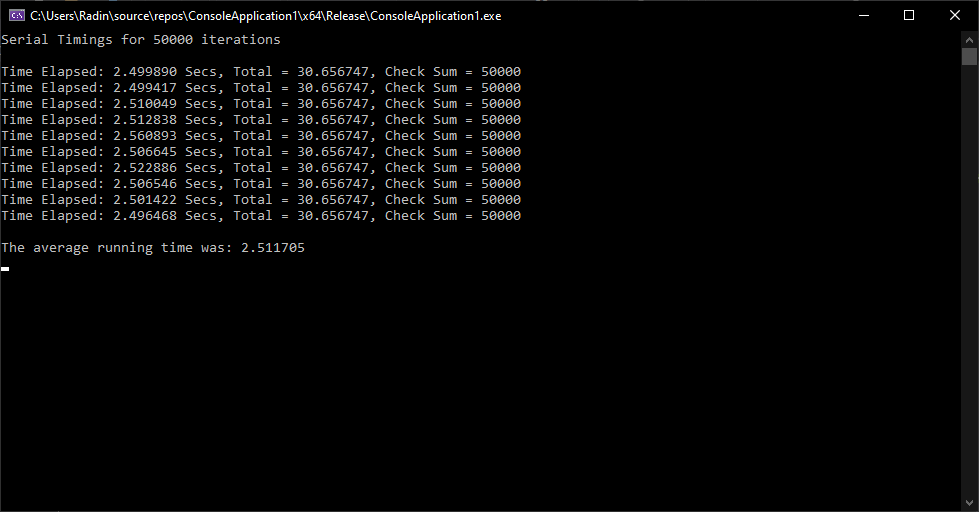
\includegraphics[width=15cm]{images/serial}
\end{center}
\caption{زمان اجرای برنامه در حالت سریال}
\label{fig:serial}
\end{figure}

%%%%%%%%%%%%%%%%%%%%%%%%%%%%%%%%
%Q1
\begin{question}
دو حلقه با شمارنده \lr{k} که به انجام محاسبات ریاضی می‌پردازند، بیشترین زمان اجرا را در این کد دارند. برای تسریع زمان اجرا، می‌توان اجراهای مختلف آن‌ها (حلقه \lr{j}) را بر روی هسته‌های مختلف موازی‌سازی کرد.
\end{question}

%%%%%%%%%%%%%%%%%%%%%%%%%%%%%%%%
%Q2
\begin{question}
به دلیل اینکه عوامل زیادی (مانند وضعیت و بار سیستم در هنگام اجرای برنامه) روی زمان اجرا تاثیر می‌گذارند، بهتر است برای اندازه‌گیری زمان اجرا به جای یک بار، چند بار برنامه را اجرا کنیم و در نهایت زمان‌های صرف شده را میانگین بگیریم.

در اینجا (در حالت سریال)، تنها زمان اجرا از اجرایی به اجرای دیگر (به دلیل گفته شده) متفاوت است. همچنین باید توجه داشت در بسیاری از موارد، ممکن است برنامه به علت داشتن ایراداتی (مانند شرایط مسابقه در برنامه‌های موازی) نتایج آن به غلط از اجرایی به اجرای دیگر تغییر کند. چنین اتفاقی نیز معمولا با چندین بار اجرا قابل کشف است.
\end{question}

%%%%%%%%%%%%%%%%%%%%%%%%%%%%%%%%
%Q3
\begin{question}
دو حالت \lr{Release} و \lr{Debug} تنها دو پیکربندی (\lr{Configuration}) مختلف برای کامپایل و اجرای برنامه‌هاست و به خودی خود مفهوم متفاوتی از هم ندارند. اما به صورت پیش‌فرض در ویژوال استودیو تفاوت‌هایی بین ویژگی‌های (\lr{Properties}) این دو پیکربندی وجود دارد. اصلی‌ترین عاملی که موجب سریع‌تر بودن حالت \lr{Release} می‌شود، فعال بودن بهینه‌سازی‌های (\lr{Optimizations}) کامپایلر، برخلاف حالت \lr{Debug}، است.

به صورت پیش‌فرض در حالت \lr{Release}، تنظیمات بهینه‌سازی کامپایلر روی حالت \lr{O2} (بیشترین بهینه‌سازی برای سرعت اجرا) است. در حالی که در حالت \lr{Debug} تنظیمات آن روی \lr{Od} (غیرفعال بودن بهینه‌سازی‌ها) است.
\end{question}

%%%%%%%%%%%%%%%%%%%%%%%%%%%%%%%%
%Q4
\begin{question}
از آنجا که اجراهای حلقه \lr{j} مستقل از هم هستند، می‌توان آن را موازی کرد. برای این کار از روش تجزیه \lr{Geometric Decomposition} و الگوی \lr{Loop Parallelism} استفاده می‌کنیم.
\end{question}

\section{مرحله دوم}

با استفاده از خط زیر، اجراهای حلقه \lr{j} را روی هسته‌های مختلف موازی‌سازی می کنیم.
\begin{latin}
\begin{lstlisting}[language=C]
#pragma omp parallel for
\end{lstlisting}
\end{latin}
مطابق شکل
\ref{fig:parallel-for}،
زمان اجرای برنامه در این حالت برخلاف انتظار بسیار بیشتر شده و به طور میانگین \textbf{۴۴/۷۲ ثانیه} است. علت این امر آن است که در این کد متغیرهای اشتراکی به شدت استفاده می‌شوند و این باعث کندی اجرا می‌شود. همچنین به علت وجود شرایط مسابقه روی این متغیرهای اشتراکی (از جمله \lr{sum} و \lr{total}) وجود دارد که باعث متفاوت بودن خروجی چاپ شده در 
اجراهای مختلف است.

\begin{figure}[ht!]
\begin{center}
	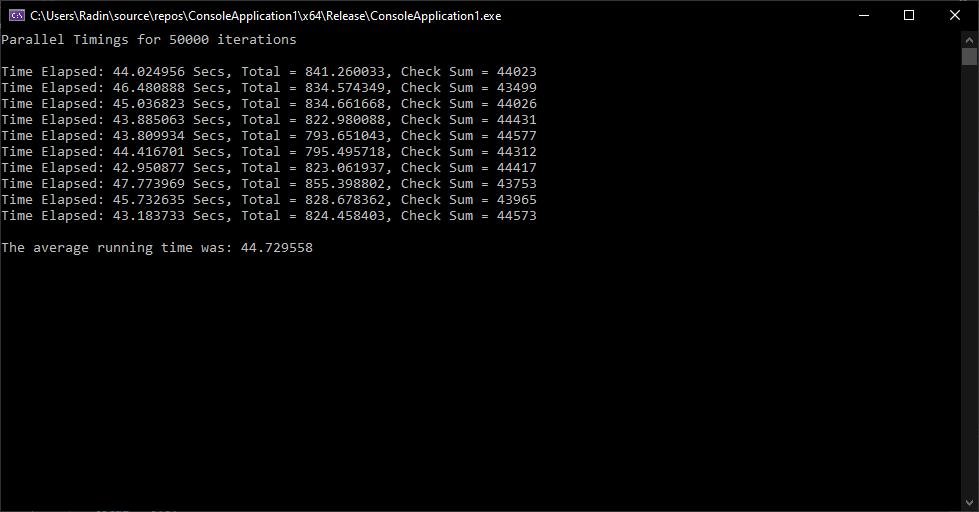
\includegraphics[width=15cm]{images/parallel-for}
\end{center}
\caption{طولانی‌تر شدن زمان اجرا و تفاوت خروجی برنامه در اجراهای مختلف به علت استفاده مکرر از متغیرهای اشتراکی و وجود شرایط مسابقه}
\label{fig:parallel-for}
\end{figure}

با محلی کردن برخی متغیرها به کمک عبارت زیر، مطابق شکل
\ref{fig:parallel-private}
می‌بینیم که سرعت اجرای برنامه به علت موازی‌سازی روی هسته‌های مختلف بیشتر شده است و به مقدار میانگین \textbf{۰/۶۴ ثانیه} رسیده است. اما همچنان خروجی برنامه به علت وجود شرایط مسابقه در اجراهای مختلف متفاوت است.

\begin{latin}
\begin{lstlisting}[language=C]
private(k, sumx, sumy)
\end{lstlisting}
\end{latin}

\begin{figure}[ht!]
\begin{center}
	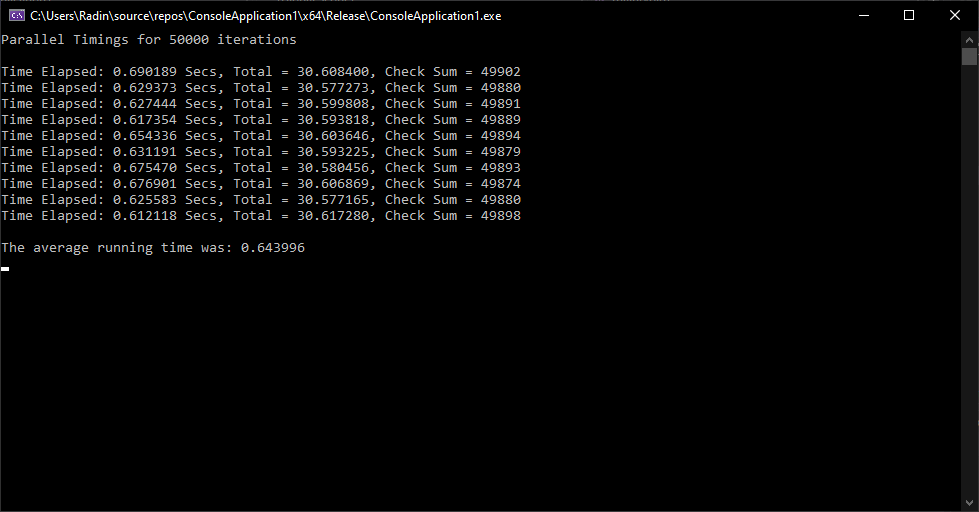
\includegraphics[width=15cm]{images/parallel-private}
\end{center}
\caption{رفع مشکل زمان اجرای طولانی برنامه با محلی کردن برخی متغیرها}
\label{fig:parallel-private}
\end{figure}

مطابق شکل
\ref{fig:parallel-critical}،
با اضافه کردن کد زیر در بخش‌هایی که روی متغیرهای \lr{sum} و \lr{total} می‌نویسند، مشکل شرایط مسابقه‌ای و متفاوت بودن نتابج اجراهای مختلف برطرف شده است.  زمان اجرای برنامه در این حالت نیز به طور میانگین \textbf{۰/۶۴ ثانیه} است.

\begin{latin}
\begin{lstlisting}[language=C]
#pragma omp critical
\end{lstlisting}
\end{latin}

\begin{figure}[ht!]
\begin{center}
	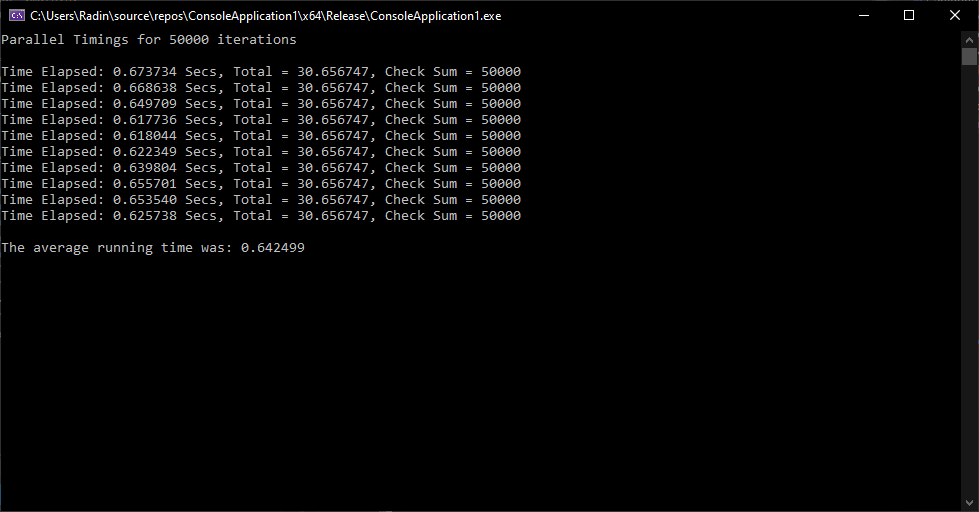
\includegraphics[width=15cm]{images/parallel-critical}
\end{center}
\caption{رفع مشکل شرایط مسابقه با استفاده از راهنمای \lr{critical}}
\label{fig:parallel-critical}
\end{figure}

با استفاده از \lr{reduction} به جای \lr{critical}، برنامه باز هم به طور میانگین در زمان
\textbf{۰/۶۴ ثانیه}
(شکل 
\ref{fig:parallel-reduction})
اجرا می‌شود.

\begin{figure}[ht!]
\begin{center}
	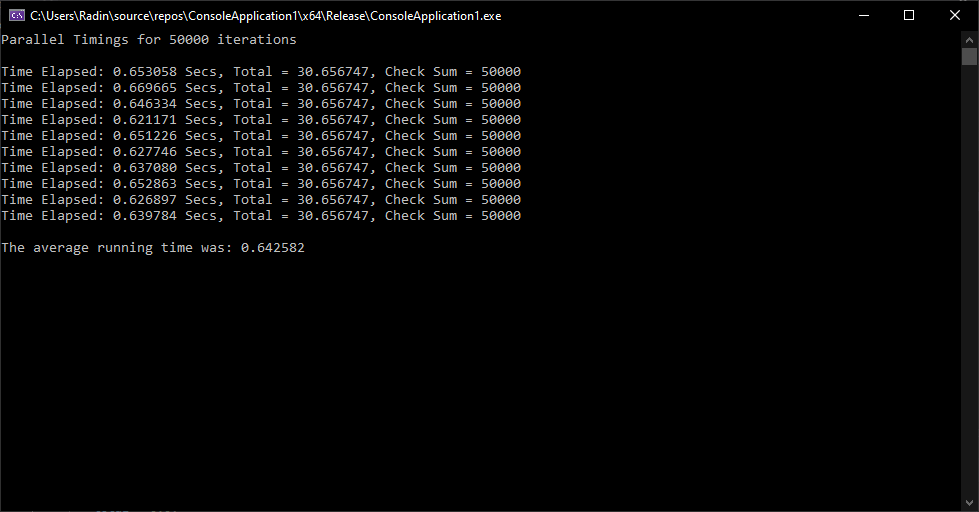
\includegraphics[width=15cm]{images/parallel-reduction}
\end{center}
\caption{رفع مشکل شرایط مسابقه با استفاده از راهنمای \lr{reduction}}
\label{fig:parallel-reduction}
\end{figure}

راه‌حل دیگر برای جلوگیری از مشکلات ناحیه بحرانی، استفاده از قفل است. با استفاده از خطوط زیر، دو قفل برای دو متغیر اشتراکی می‌سازیم و ناحیه‌های بحرانی آن‌ها را با این قفل‌ها محافظت می‌کنیم.

\begin{latin}
\begin{minipage}{\linewidth}
\begin{lstlisting}[language=C]
omp_lock_t sum_lock, total_lock;
omp_init_lock(&sum_lock);
omp_init_lock(&total_lock);
\end{lstlisting}
\end{minipage}
\end{latin}

مطابق شکل
\ref{fig:parallel-lock}،
مشکل ناحیه بحرانی با استفاده از همگام‌سازی سطح پایین نیز قابل حل است.

\begin{figure}[ht!]
\begin{center}
	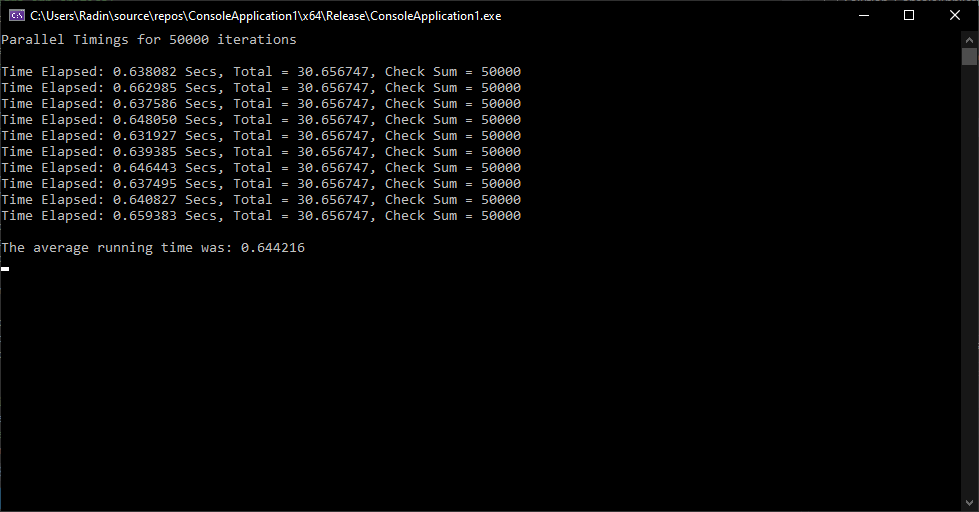
\includegraphics[width=15cm]{images/parallel-lock}
\end{center}
\caption{استفاده از همگام‌سازی سطح پایین (\lr{Lock}) برای محافظت از ناحیه بحرانی}
\label{fig:parallel-lock}
\end{figure}

\setcounter{mynumber}{1}
%%%%%%%%%%%%%%%%%%%%%%%%%%%%%%%%
%Q1
\begin{question}

\end{question}


\end{document}
